\begin{center}
  \Large
  \textbf{BIOGRAFI PENULIS}
\end{center}

\addcontentsline{toc}{chapter}{BIOGRAFI PENULIS}

\vspace{2ex}

\begin{wrapfigure}{L}{0.3\textwidth}
  \centering
  \vspace{-3ex}
  % Ubah file gambar berikut dengan file foto dari mahasiswa
  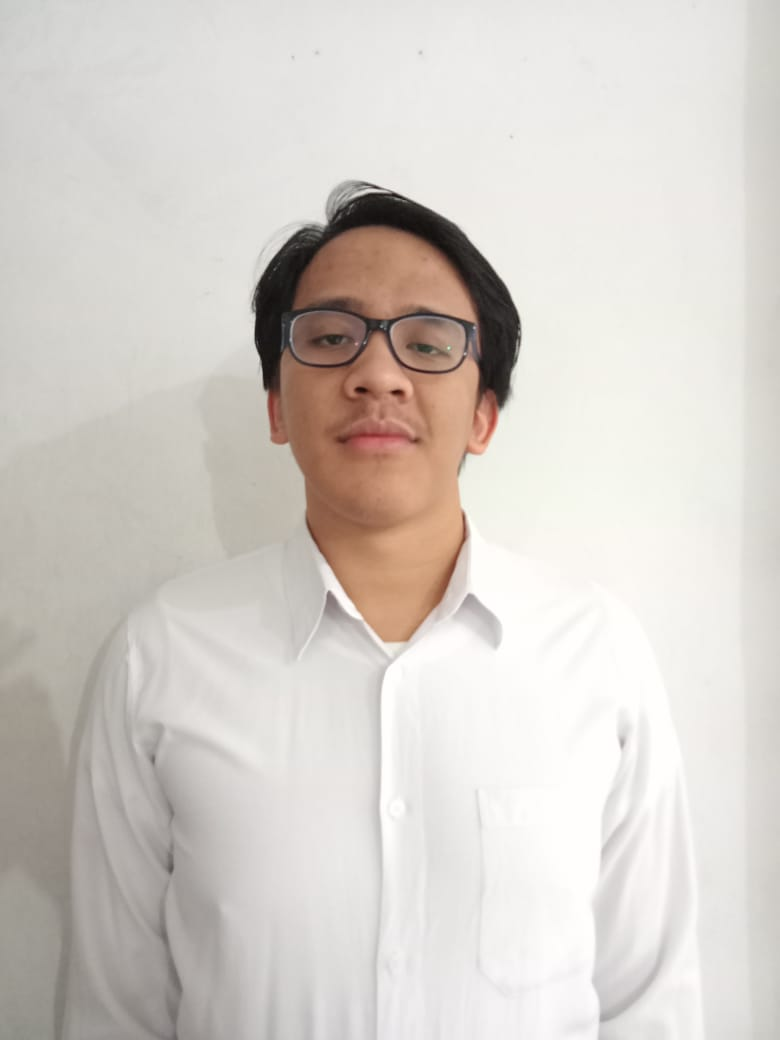
\includegraphics[width=0.3\textwidth]{gambar/John.jpeg}
  \vspace{-4ex}
\end{wrapfigure}

% Ubah kalimat berikut dengan biografi dari mahasiswa
\name{}, lahir pada tanggal 30 Juni 2001 di Lahat, Sumatera Selatan, merupakan anak kedua dari 3 bersaudara. 
Penulis telah menempuh pendidikan formal yaitu di TK Pembina HKBP Tarutung, SDS Latihan HKBP Pearaja Tarutung, SMPN 2 Tarutung dan SMAS Unggul Del. 
Setelah lulus dari SMA pada tahun 2019, penulis mengikuti Ujian Tulis Berbasis Komputer (UTBK) dan diterima di Departemen \department{} FTEIC - ITS pada tahun 2019 dan terdaftar resmi dengan Nomor Pokok (NRP) 07211940000040.

Di Departemen Teknik Komputer, penulis aktif mengikuti beberapa kegiatan Seminar yang diselenggarakan oleh Departemen dan Himpunan Mahasiswa Teknik Komputer (HIMATEKKOM).
Penulis ikut aktif menjadi bagian dalam organisasi dan event yang diselenggarakan Departemen \department{}, seperti HIMATEKKOM dan MAGE (Multimedia and Game Event).
Penulis juga mendapat pengalaman dari Studi Independen yang diselenggarakan oleh Kampus Merdeka, yaitu Bangkit Academy 2022, dan selama hampir 6 bulan, penulis mendalami pengetahuan dibidang \emph{Cloud Computing Path}.
